\documentclass{beamer}

\usepackage{graphics}

\title{Introduction to Machine Learning}
\author{Joseph P. Vantassel}
\institute{The University of Texas at Austin}
\date{2021}

\begin{document}

\frame{\titlepage}


\begin{frame}

\frametitle{Terminology}

What are the differences between Artificial Intelligence, Machine Learning, and Deep Learning?

\begin{center}
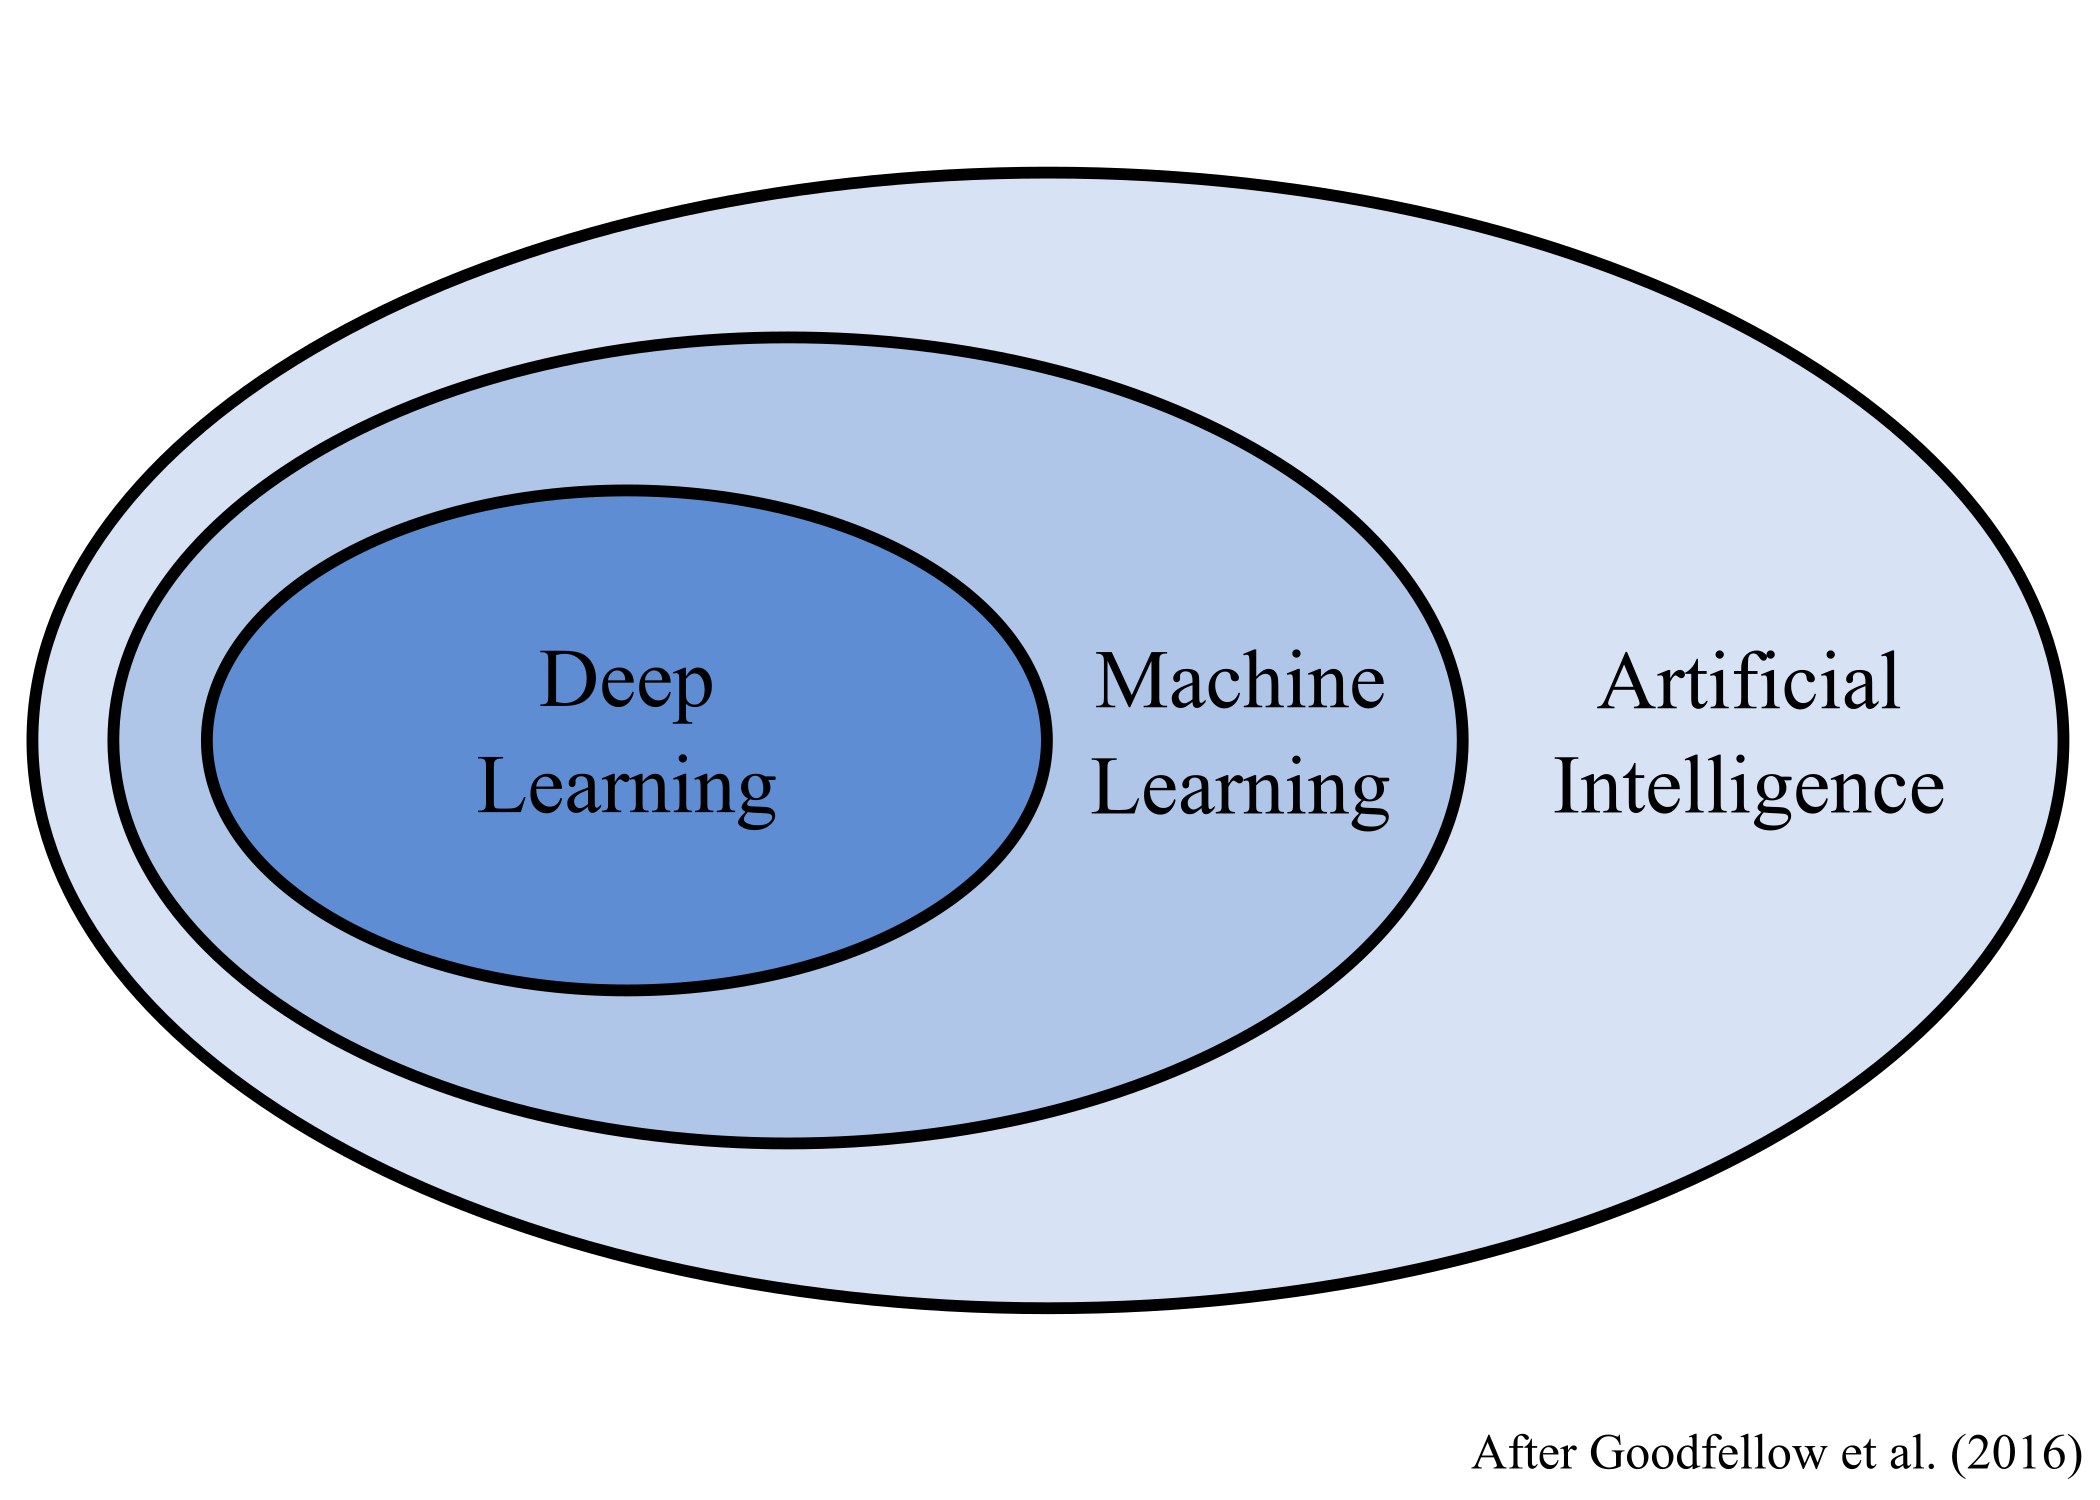
\includegraphics[height=5cm]{figs/0-ai_ml_dl_diagram.png}
\end{center}

\end{frame}


\begin{frame}

\frametitle{Artifical Intelligence (AI)}

\begin{itemize}
    \item Started in 1950's.
    \item Includes algorithms that allows computers to act intelligently.
    \item Early work focused on rule-based controllers.
\end{itemize}

\end{frame}


\begin{frame}

\frametitle{Machine Learning (ML)}

\begin{itemize}
    \item Started in 1980's.
    \item Includes algorithms that allows computers to teach themselves.
    \item Classic Examples:
    \begin{itemize}
        \item Support Vector Machines (SVM)
        \item K - Nearest Neighbor Classification
    \end{itemize}
\end{itemize}

\begin{block}{Definition - \textit{Mitchel T. (1997)}}
    ``Machine learning describes the process by which a computer adapts
    from experience \textbf{E}, on task \textbf{T}, to improve
    performance \textbf{P}.''
\end{block}

\end{frame}


\begin{frame}

\frametitle{Deep Learning (DL)}

\begin{itemize}
    \item Started in 2010's.
    \item Special subclass of ML algorithm with potential for high-dimensional representations.
    \item Classic Examples:
    \begin{itemize}
        \item Multi-Layer Perceptrons (MLP)
        \item Convolutional Neural Networks (CNN)
        \item Long Short-Term Memory (LSTM)
    \end{itemize}
\end{itemize}

\end{frame}

\begin{frame}

\begin{block}{Definition - \textit{Mitchel T. (1997)}}
    ``Machine learning describes the process by which a computer adapts
    from experience \textbf{E}, on task \textbf{T}, to improve
    performance \textbf{P}.''
\end{block}
    
\end{frame}

\end{document}